\chapter{MemoryStroop: Concept, Design and Implementation}
\label{ch:development}

In this chapter, it is presented the guidelines of the implementation with the requirements' analysis, the technical aspects of its development, and the general work  (this research is only presented in the next chapter, `Experiment'). After presenting requirements' basis as it was indicated in previous chapter, it is time to consolidate for validating it with its targeted final users, in this case, ADHD children. As underlined before, a gamified application has to deal, to balance funny features with serious aims in order to turn practical but awful tasks more pleasant. This is the main principle of this thesis, that can be shown in every section of the present chapter, where it could finally evaluate the core features.

\section{Introduction and Requirements}

The requirements are based in the psychologists' perceptions about a another gamified application for ADHD children and in an idea collected from a scientific article of Psychology. First of all, it is necessary explain the fundamental contribution for the present work.

\subsection{Requirement Prospection}

It was pointed out, mainly by psychologists' opinions, some necessities have to be achieved. In general they approved it and they had critical look on the working of the described software as meaningful treatment. In general they approved and viewed with good eyes the use of the said software as mean of the treatment. But some of them manifested the following points for improving in newer version of software: first, the gaming has too much conflicting stimuli in some of its levels, secondly general performance report is needed and thirdly moving targets the player. Understanding the former application, it is possible to draw similarities and contrasts with the present application. In summary, most of ADHD games implement gaming centered in matching  (like the third step of test of John Ridley Stroop (shown in Chapter \ref{ch:ADHD}), but more influenced by Golden Stroop modality) of a color's name to an ink but most of times in a situation of conflicting stimuli, mainly a conflict between the color name and its background ink. Along eight levels the player/patient executes progressively-difficult tasks, from the simplest matching of a color name and its ink to a difficult scenario with a series of adverse stimuli in the last level.

\subsection{Defining Requirements}

A general score with the responding time and hit rates was implemented to the satisfaction of the requirement expressed by the some psychologists that evaluated another application \citep{Villa}. Then the following requirements systematize and consolidate their impressions, according to some strict software engineering paradigms, including the functional and non-functional ones. The latter was disposed according to the patterns of ISO9126's norms.


\begin{table}[htp] % The `h` means place the table here. The exclamation mark tells Latex to really try to place the table here. Use with caution! 
	
	\begin{center}
		\scalebox{0.85}{
			\begin{tabular}{ l  l  l  l }
				\hline
				\textbf{Number} & \textbf{As a <role>} & \textbf{As a <goal>} & \textbf{As a <result>} \\
				\hline \hline
				1 & Player & access game & select new game\\
				1.1 & Player & give the name & write his/her name \\
				1.2 & System & generate board 
				& dispose `Stroop' memory cards \\
				2 & Player & seek color name combination  & pass levels\\
				2.1 & System &  manage hits and mistakes & improve difficulty slightly \\
				2.2  & Player & advance levels until the end & conclude gaming \\
				3 & Psychologist & see statistics &  must store and see player's name and numbers
				\\
				\hline \hline
			\end{tabular}}
		\end{center}
		\label{tab:highuserstories}
		\caption{Table for the all functional requirements}
		
The functional requirements comprises each of game events and human interaction with the system. They will be verified on Chapter \ref{ch:experiment} alongside the presentation of the practical research with computer science specialists.

	\end{table}
	
	\begin{table}[h!]

		
		\begin{center}
			\scalebox{0.6}{%
				\begin{tabular}{ l  l  l }
					\hline
					\textbf{Number} & \textbf{Requirements} & \textbf{Quality in use} \\
					\hline \hline	
					\textbf{Functionality} & & \\
					F1 & The player should have only option to follow the game levels & Consistency\\
					F2 & The system should each level's statistics & Consistency\\
					\hline
					\textbf{Usability} & & \\
					U1 & A new player should be able to use the system after less than 5 minutes training & Learnability\\
					U2 & The system should be perceived as easy to use by at least 85\% of its users & Understandability \\
					\hline
					\textbf{Maintainability} & & \\
					M1 & The system should be easy to extend and modify & Changeability\\ % Make measurable
					\hline
					\textbf{Portability} & & \\
					P1 & The system should run on the majority of used Android devices without additional resources & Installability\\
					\hline \hline
				\end{tabular} }
			\end{center}
			\label{tab:NonFuncReq}
			\caption{Table for all non-functional requirements}
		\end{table}


\subsection{Technologies Applied to Software Development}
		
The working technologies are only the basic infrastructure for software development. The codification of this mobile software was made in Java programming language driven by an Android mobile operating system. It was used the Android Studio framework in version 1.5.1 for the development. Implementing gradle, the package manager for android projects, and some other frameworks too, the lint prototypes validator and OpenJDK 7 (Java Developer Kit) for Java programming language infrastructure on a Debian 8 (Jessie) operating system desktop for development. \footnote{Although Google warns that using Open JDK instead the Oracle proprietary JDK may let problems to application, but there are no problems related to this in the application.} 
		
What differs from traditional Java for desktops or other mobile platfoms is that Android has some specific functions, like: Calling device resources or sensors.  And it runs in another virtual machine than common Java called: the Dalvik Virtual Machine. Android has a stack of operating system levels, beginning from Linux kernel, passing to a device-components layer and other levels until the graphic user interface domain. Which you can see in the Figure \ref{android}.
		
		\begin{figure}[htp]
			\begin{center}
				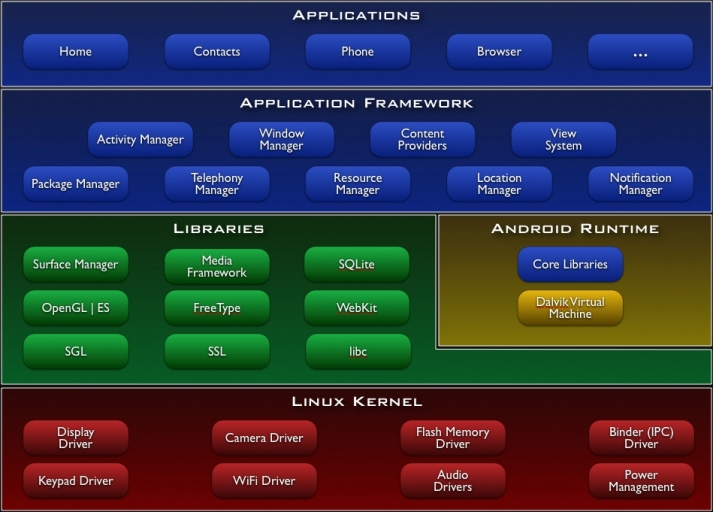
\includegraphics[scale=0.65]{chapters/desenvolvimento/img/android.jpeg}
				\caption{Android Operating System basic layer structure \citep{1_fundamentals_2015}.}
				\label{android}
			\end{center}
		\end{figure}
		
The Android environment was chosen especially, because it is currently the most used platform around the world. Particularly in Brazil, where this study was designed, and most of 80\% of mobile devices are based on  Android, which I mentioned earlier in the introduction. The native application approach, compared to other types of hybrid approaches. Like cross-compile one, was here used to explore all of its possibilities from native devices standard computational resources. In this way, it will be so difficult to develop many native applications driven for each mean mobile device's operating system, like IOs or Windows Phone, because it’s demanding more time and resources than a single coursework subject could afford.

		
The present application was designed for Android, to achieve a greater number of potential users. But the experiment, which was designed for this research. It only comprise a controlled, reduced group of people, because the software is an experimental application. Although there are other versions offered for free in the App store from Google, none of them seems to train working memory skills, which containing dozens of millions of mobile applications with the most different finalities, but the platform from Android is more accessible for developing, compared to platforms like IOs or Blackberry. Because these systems need a considerable number of environmental requirements, which is an exigence  of a Mac computer to program in Objective-C or Swift (programing languages for applications in IOs). This turns programming more difficult to be achieved during the time needed for concluding a undergraduate thesis. 

There are a couple of reasons to adopt the Android environment for developing the application of this research. Mainly because of its popularity in Brazil and the relative practicality for development. The application is compatible from Android called ‘KitKat’(version 4.4) to the most recent versions (the most stable recent version in this moment is version 6 called ``Marshmallow''). Which yields a compatibility ratio of 74\% of Android devices on a word-wide perspective, according to recent data \citep{android-official}.The implementation also is driven to treat different resolutions of devices, using scalable images and other strategies, as it will be discussed soon. In this case, tablets and smart-phones with different dimensions like Galaxy Nexus or Moto G and son could run as well the application presented here. 

To develop the game core features, the Libgdx Java library engine was used. This is a free software engine that allows anyone to program simple games  in 2D or 3D for various platforms, including Android. The proposed application ‘Mememory Stroop’ is combining Libgdx to android native code and  has proper guidelines for this system. Libdgx offers a large set of facilities to develop games better for Android. Maybe the most important thing is: Its simplicity of operations, their basic project's architecture and the by both shared high integration Java programming language: Syntax and so on. 

Additionally, Android Studio IDE could easily manage Libgdx projects with gradle and implement extra native code as well. Furthermore, this Java game engine has powerful resources to implement: Game textures, sprites, events, loops, input-getting, abstract and non-abstract screens, and other features that let game development and gamification more accessible to non-specialists in that area.

		
\section{Application Architecture}

As mentioned before, other ADHD gamification apps comprise multiple conflict situations in a game that appeared undesirable to some psychologists. So these extensions sets of conflicting mechanisms was replaced by only two conflicting stimuli: The classical Stroop Test, and a fixed memory game board, in order to promote a more focused set of stimuli. It was added in the present application. That is why the application is called: MemoryStroop. \footnote{From many memory game approaches, the present application follows as a improved fork of Mathias Lux proposal avalaible in https://github.com/dermotte/memory-game-android and licensed by Apache 2.0 license.}.  All negative stimuli that remained on previous version, like ``game over'' event, are put aside: only positive stimuli such as commemorative music effects are implemented, no negative stimuli at all. The application class model is shown in the figure \ref{uml}. and explained next.
		
				\begin{figure}[htp]
					\begin{center}
						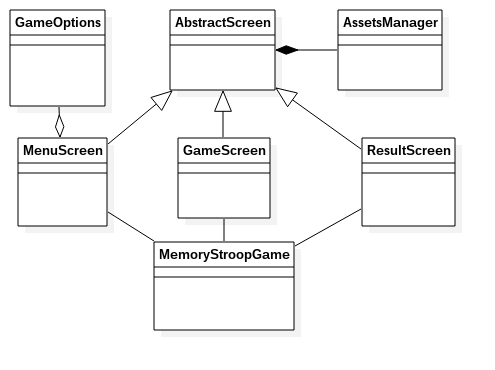
\includegraphics[scale=0.65]{chapters/desenvolvimento/img/uml_2.png}
						\caption{Elementary exhibition of class diagram using StarUML tool.}
						\label{uml}
					\end{center}
				\end{figure}
		
The main class is the MemoryStroopGame, in which the engine is put in a loop to provide touch inputs and manage each reaction of game features like right or wrong card combination, level changing and so on. The screen classes are extended by a abstract class that defines is their common attributes and methods. The class GameScreen receives touches from tablet or smart screen and sends them to the MemoryStroopGame class. Besides it is possible see the game implementation's architecture of Libgdx Java classes and extra native android class, that implements TXT exportation of game statistical data. This functionality is called by a separate android java class that is not shown on main diagram. \textit{Memory Stroop} game is not designed to be played lonely by the young patients but instead this it is designed to be played in monitored way, in which the psychologist may observe actions and after child playing see the statistic results. This process is drawn in the following figure as sequence diagram \ref{sequence}.
		
						\begin{figure}[htp]
							\begin{center}
								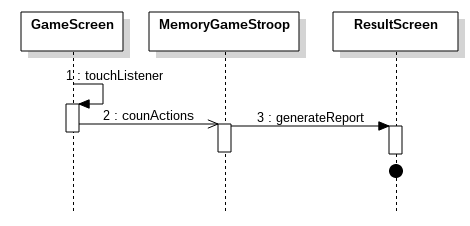
\includegraphics[scale=0.65]{chapters/desenvolvimento/img/sequence.png}
								\caption{Main flux of game loop in a sequence diagram using StarUML tool.}
								\label{sequence}
							\end{center}
						\end{figure}

\subsection{Game Workflow}

The first screen of the game is the main menu, after that is the main menu, in which the player could switch off sound effects or consult the credits.

						\begin{figure}[htp]
							\begin{center}
								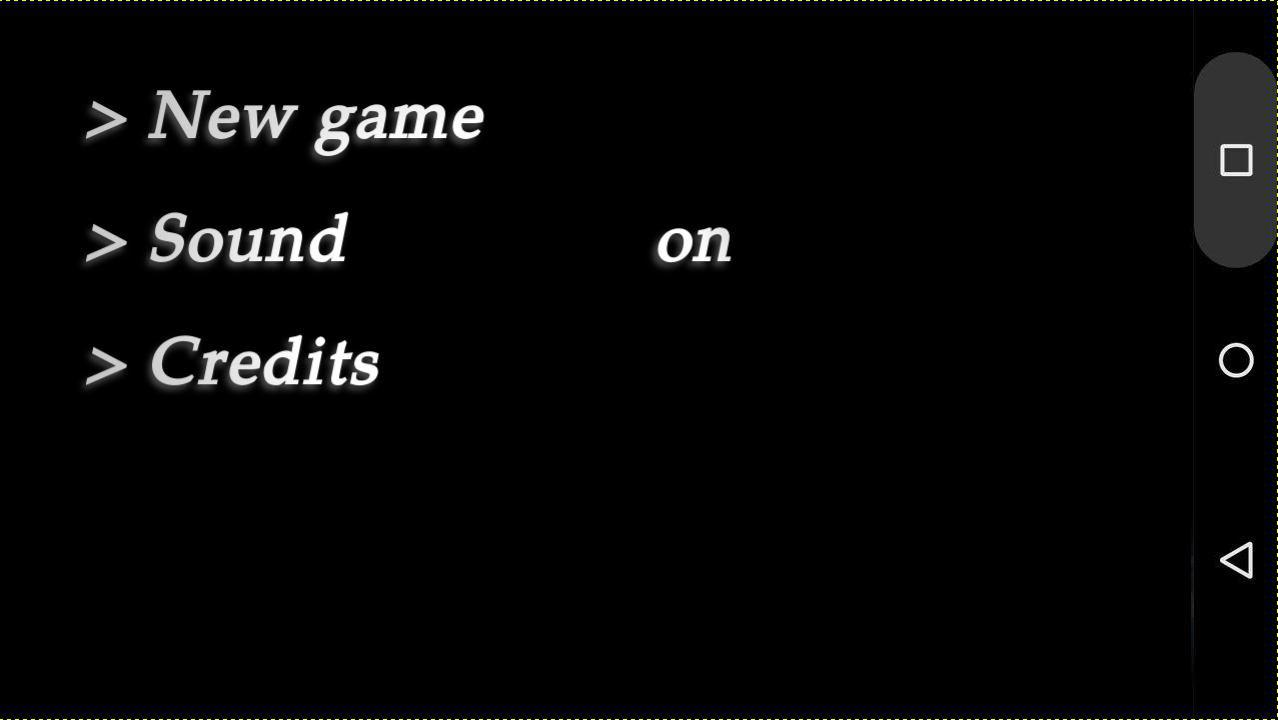
\includegraphics[scale=0.35]{chapters/desenvolvimento/img/menu.png}
								\caption{Main menu.}
								\label{menu}
							\end{center}
						\end{figure}
		
After selecting new game option the player is asked to fill its name and the first level begins. In the first level some cards has some figures of fruits or cars to facilitate to children the understanding about how to match `Stroop Effect' Cards in this and in the next levels. In this level the Stroop cards has only a white background to facilitate even more. Figure \ref{lv1} shows the image of the level 1 with the commemoration message that appears when players win.

						\begin{figure}[htp]
							\begin{center}
								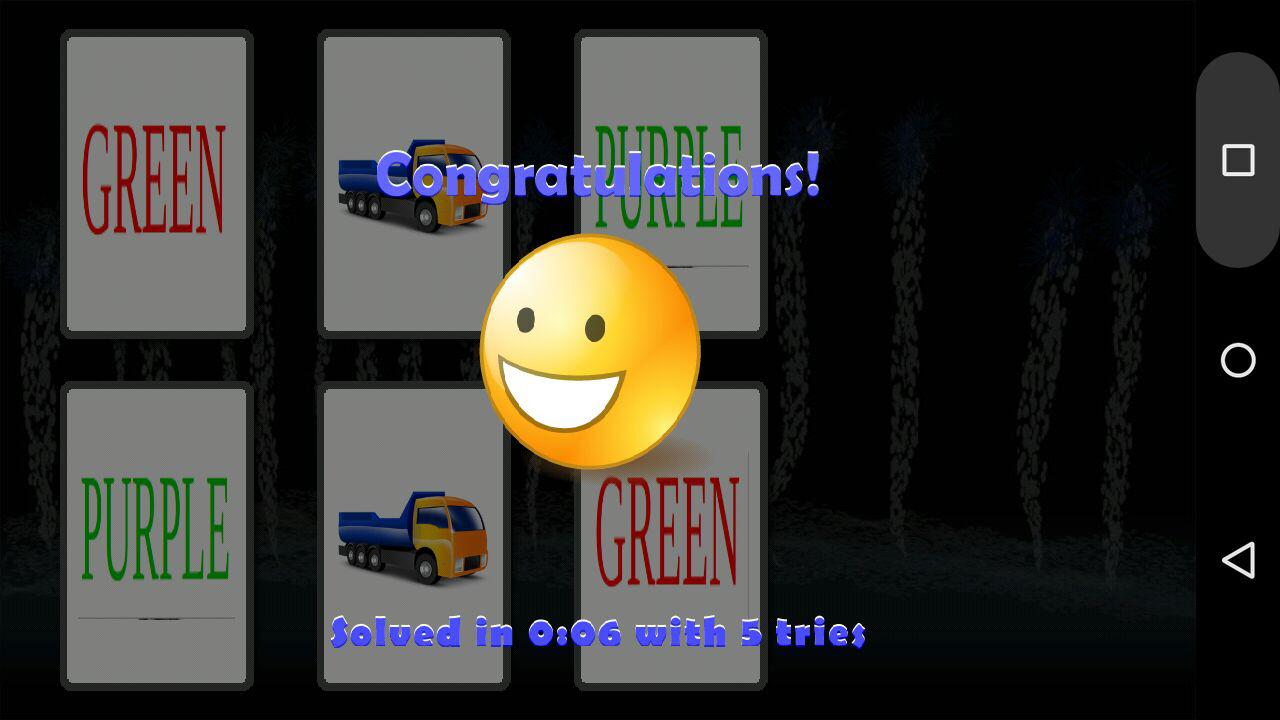
\includegraphics[scale=0.35]{chapters/desenvolvimento/img/memorystroop0.jpg}
								\caption{Level 1.}
								\label{lv1}
							\end{center}
						\end{figure}

The second level increments the difficult by removing images. The number of cards is maintained. Figure \ref{lv2} exposes this second level.

						\begin{figure}[htp]
							\begin{center}
								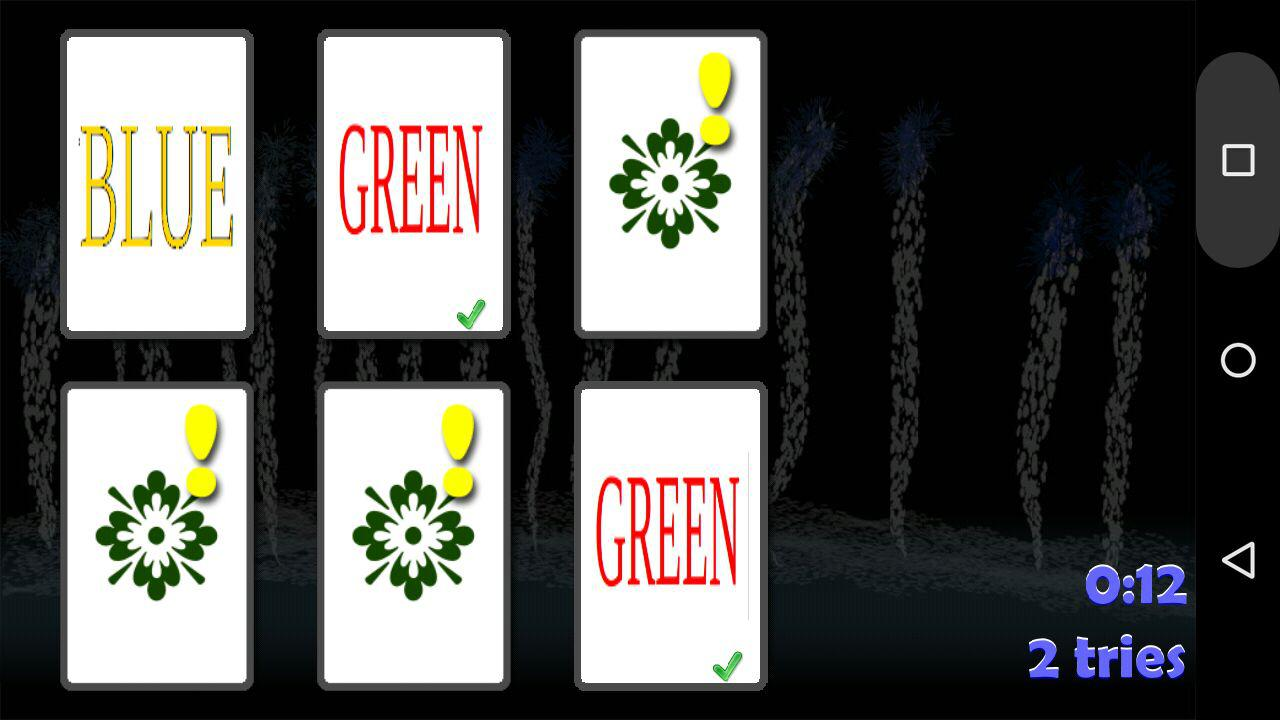
\includegraphics[scale=0.35]{chapters/desenvolvimento/img/memorystroop.jpg}
								\caption{Level 2.}
								\label{lv2}
							\end{center}
						\end{figure}

The third level become more difficult by the increase of card quantity, and, sometimes, the background color of cards became different among them randomly, but after matching they return to the normal white background. Figure \ref{lv3} exposes this third level with 18 cards.


						\begin{figure}[htp]
							\begin{center}
								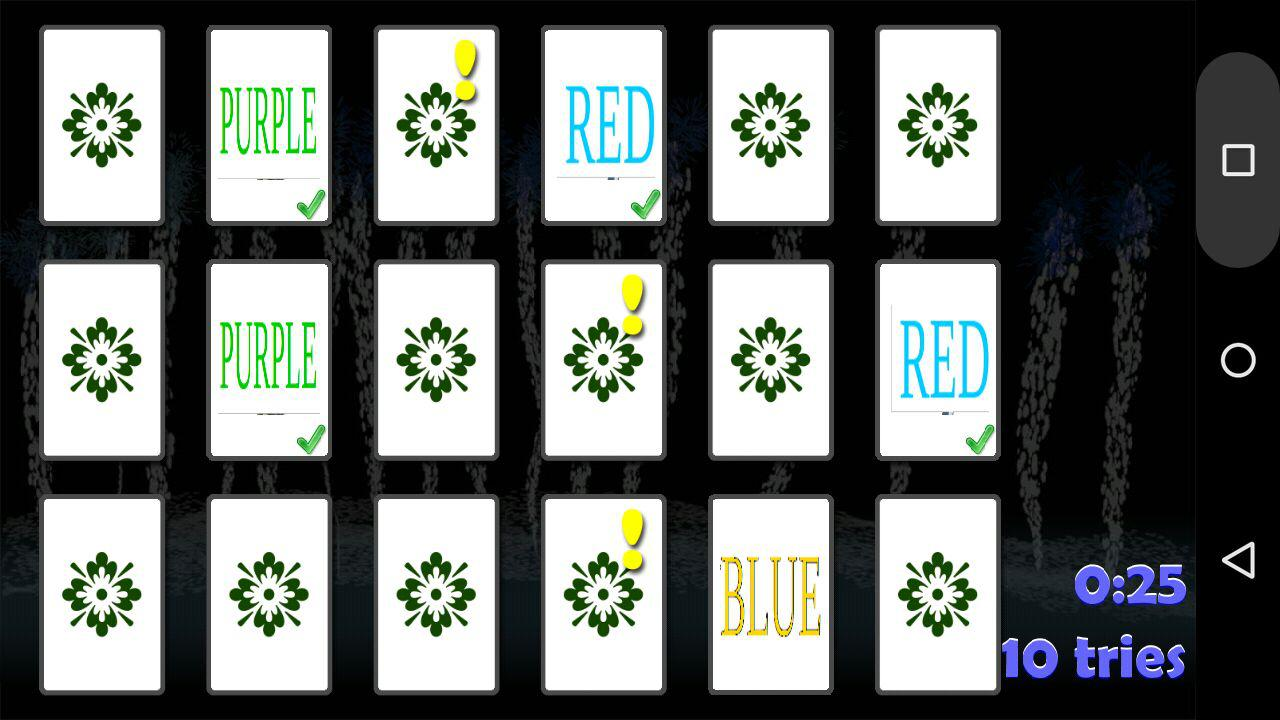
\includegraphics[scale=0.35]{chapters/desenvolvimento/img/memorystroop2.jpg}
								\caption{Level 3.}
								\label{lv3}
							\end{center}
						\end{figure}

The fourth and last level only increment the quantity of cards. Figure \ref{lv4} exposes this third level's cards on the moment of beginning of cards distribution, 32 at total.

						\begin{figure}[htp]
							\begin{center}
								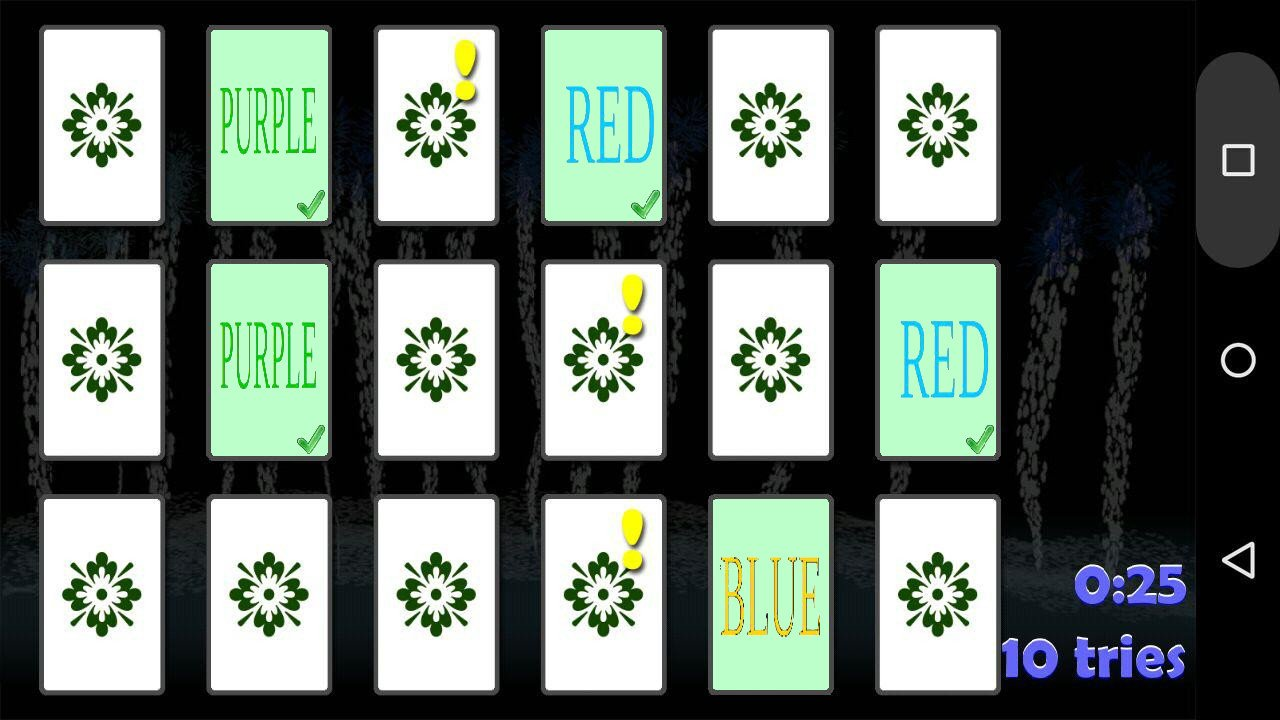
\includegraphics[scale=0.25]{chapters/desenvolvimento/img/memorystroop4.jpg}
								\caption{Level 4.}
								\label{lv4}
							\end{center}
						\end{figure}


\section{Summary}
		
The point was to explain the following aspects: The computational settings and the implementation of MemoryStroop. The first necessity referred to the definition of requirements (this came from a previous application and research) evolved improving some of the main features of other application presented to the psychologists for this application and research. The main requirement of those psychologists was the necessity to offer a limited set of conflicting stimuli in the Stroop Effect during the game. In short, the functional and non-functional  requirements that includes all implementations.  At the last point, the architectural and practical engine of the gamification was presented to the reader.